\scanpage{28}

% Layout anchors the long rules to the correction list and the foot note.
% Coordinates refer to the whole image in original pixels.
% No mathematical display or diagram occurs on the sheet.
\figure{
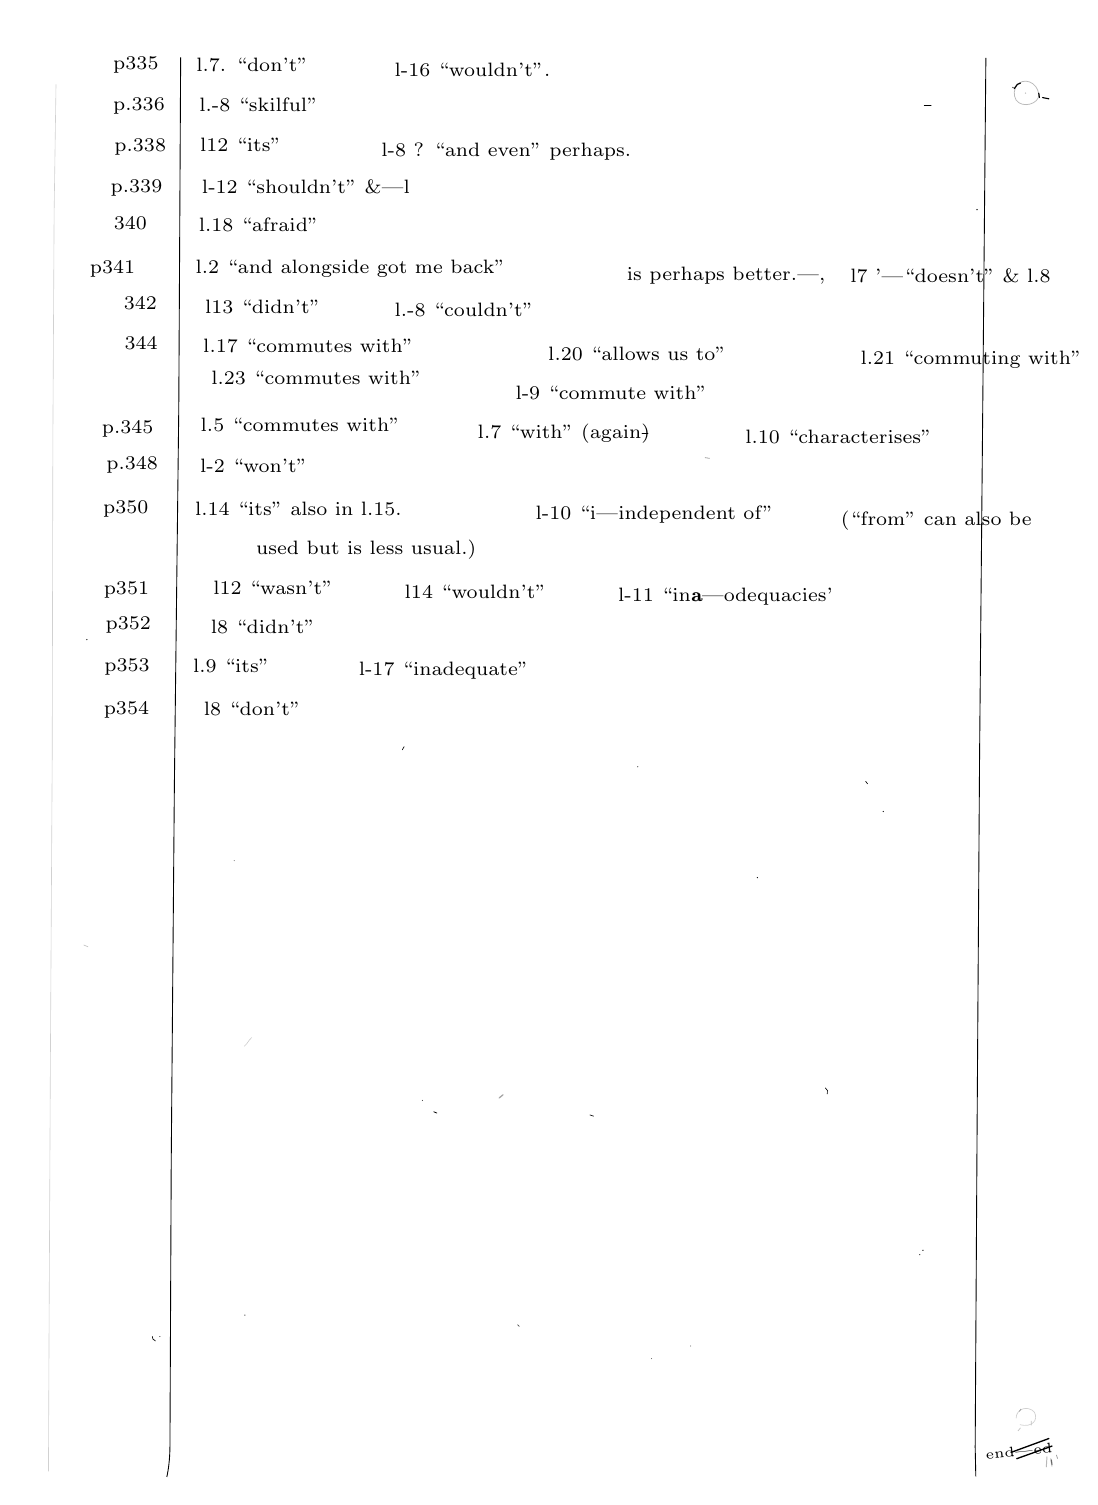
\begin{tikzpicture}[x=.008cm,y=-.008cm,every node/.style={anchor=base west,inner sep=0pt,font=\scriptsize}]
\path[use as bounding box] (15,45) rectangle (1670,2347);
% left_rule
\draw[line width=.32pt] (258,92)--(255,650)--(248,1250)--(243,1850)--(241,2296)..controls(241,2321)and(238,2338)..(236,2347);
% right_rule
\draw[line width=.32pt] (1537,93)--(1532,650)--(1527,1200)--(1523,1800)--(1520,2300)--(1521,2346);
% faint_left_trace
\draw[black!18,line width=.22pt] (60,135)--(57,340)--(55,700)--(54,1200)--(51,1700)--(49,2110)--(48,2338);
% Text block 01
\node at (150,111) {p335};
\node at (282,115) {l.7. ``don't''};
\node at (597,122) {l-16 ``wouldn't''.};
% Text block 02
\node at (150,176) {p.336};
\node at (287,178) {l.-8 ``skilful''};
% Text block 03
\node at (152,242) {p.338};
\node at (288,241) {l12 ``its''};
\node at (576,250) {l-8 ? ``and even'' perhaps.};
% Text block 04
\node at (146,307) {p.339};
\node at (291,309) {l-12 ``shouldn't'' \deleted{\unsure{\&|l}}};
% Text block 05
\node at (151,365) {340};
\node at (286,369) {l.18 ``afraid''};
% Text block 06
\node at (113,435) {p341};
\node at (281,436) {l.2 ``and alongside \uline{got me} back''};
\node at (966,447) {is perhaps better\unsure{.|,}};
\node at (1321,449) {l7 \unsure{'|``}doesn't'' \& l.8};
% Text block 07
\node at (167,492) {342};
\node at (296,499) {l13 ``didn't''};
\node at (597,503) {l.-8 ``couldn't''};
% Text block 08
\node at (168,556) {344};
\node at (293,561) {l.17 ``commutes with''};
\node at (841,574) {l.20 ``allows us to''};
\node at (1337,580) {l.21 ``commuting with''};
% Text block 09
\node at (306,611) {l.23 ``commutes with''};
\node at (789,635) {l-9 ``commute with''};
% Text block 10
\node at (132,689) {p.345};
\node at (289,687) {l.5 ``commutes with''};
\node at (729,698) {l.7 ``with'' (again\tikz[baseline=(againcloseB28.base)]{\node[anchor=base west,inner sep=0pt] (againcloseB28) at (0,0) {)};\draw[line width=.45pt,line cap=round] (.16ex,.6ex)--(.82ex,.6ex);}};
\node at (1154,705) {l.10 ``characterises''};
% Text block 11
\node at (139,747) {p.348};
\node at (288,751) {l-2 ``won't''};
% Text block 12
\node at (134,817) {p350};
\node at (280,820) {l.14 ``its'' also in l.15.};
\node at (821,827) {l-10 ``\unsure{\uuline{i}|\uline{i}}ndependent of''};
\node at (1306,835) {(``from'' can also be};
\node at (377,882) {used but is less usual.)};
% Text block 13
\node at (135,945) {p351};
\node at (309,946) {l12 ``wasn't''};
\node at (613,951) {l14 ``wouldn't''};
\node at (952,957) {l-11 ``in\tikz[baseline=(oldaB28.base)]{\node[inner sep=0pt] (oldaB28) {\deleted{\unsure{a|o}}};\node[anchor=base west,inner sep=0pt] at ([xshift=.12ex]oldaB28.base west) {a};}dequacies'};
% Text block 14
\node at (138,1001) {p352};
\node at (305,1007) {l8 ``didn't''};
% Text block 15
\node at (136,1067) {p353};
\node at (277,1069) {l.9 ``its''};
\node at (540,1074) {l-17 ``inadequate''};
% Text block 16
\node at (135,1136) {p354};
\node at (294,1138) {l8 ``don't''};
% upper_right_loop
\draw[black!27,line width=.28pt] (1586,137)..controls(1596,123)and(1619,131)..(1621,151)..controls(1622,166)and(1595,174)..(1585,160)..controls(1580,151)and(1582,143)..(1586,137);\draw[line width=.42pt,line cap=round] (1582,142)--(1587,135)--(1592,133) (1621,149)--(1622,156) (1627,156)--(1637,158);\fill (1580,140) circle[radius=1.1];\fill[black!25] (1600,149) circle[radius=1.2];
% upper_short_dash
\draw[line width=.25pt,line cap=round] (1439,169)--(1450,169);
% point_beside_rule
\fill (1523,334) circle[radius=1.15];
% low_dash_345
\draw[black!45,line width=.22pt,line cap=round] (1091,728)--(1098,729);
% left_point_352
\fill (109,1017) circle[radius=1.05];
% blank_slash_01
\draw[line width=.22pt,line cap=round] (610,1192)--(613,1187);
% blank_point_02
\fill[black!70] (984,1219) circle[radius=.9];
% blank_slash_03
\draw[line width=.23pt,line cap=round] (1346,1242)--(1349,1246);
% blank_point_04
\fill (1374,1290) circle[radius=1.0];
% blank_point_05
\fill[black!65] (343,1368) circle[radius=.8];
% blank_point_06
\fill (1174,1395) circle[radius=1.05];
% blank_faint_dash_07
\draw[black!27,line width=.22pt] (104,1502)--(111,1505);
% blank_faint_curve_08
\draw[black!20,line width=.22pt] (359,1663)..controls(365,1658)and(365,1654)..(371,1649);
% blank_curve_09
\draw[line width=.23pt] (1282,1729)..controls(1286,1731)and(1286,1735)..(1285,1739);
% blank_gray_mark_10
\draw[black!35,line width=.48pt,line cap=round] (764,1745)--(770,1740);
% blank_point_11
\fill[black!75] (642,1749) circle[radius=.9];
% blank_mark_12
\draw[line width=.27pt,line cap=round] (660,1767)--(665,1769);
% blank_dash_13
\draw[line width=.22pt,line cap=round] (908,1772)--(914,1774);
% blank_two_points_14
\fill (1437,1987) circle[radius=1.0];\fill (1432,1994) circle[radius=.9];
% blank_point_15
\fill (360,2090) circle[radius=.95];
% blank_mark_16
\draw[black!70,line width=.22pt] (793,2105)--(796,2108);
% blank_left_cluster_17
\draw[line width=.25pt,line cap=round] (213,2124)--(214,2128)--(218,2131);\fill (225,2124) circle[radius=.8];
% blank_point_18
\fill[black!65] (1068,2139) circle[radius=.8];
% blank_point_19
\fill[black!65] (1006,2159) circle[radius=.8];
% lower_faint_loop
\draw[black!18,line width=.25pt] (1585,2254)..controls(1585,2238)and(1604,2233)..(1614,2244)..controls(1621,2257)and(1610,2269)..(1591,2264);\draw[black!40,line width=.25pt] (1590,2243)--(1593,2239);\draw[black!24,line width=.25pt] (1609,2258)--(1609,2265) (1592,2269)--(1588,2274);
% lower_pendant_marks
\draw[black!28,line width=.35pt,line cap=round] (1634,2315)--(1633,2331) (1640,2318)--(1642,2330);\draw[black!60,line width=.4pt,line cap=round] (1641,2320)--(1642,2327);\draw[black!40,line width=.25pt] (1649,2312)--(1651,2318);
% Bottom-right cancelled marginal word; interior letters remain doubtful.
\node[anchor=base east,rotate=6,font=\tiny,inner sep=0pt] (footwordB28) at (1644,2308) {\deleted{\unsure{end|ed}}};
\draw[line width=.48pt,line cap=round] (1577,2308)--(1637,2286) (1586,2318)--(1642,2298);
\end{tikzpicture}
}

% archive sheet number: 27
